\documentclass[tikz,border=10pt]{standalone}
\usepackage{tikz}
\usetikzlibrary{angles,quotes,calc,intersections}

\begin{document}
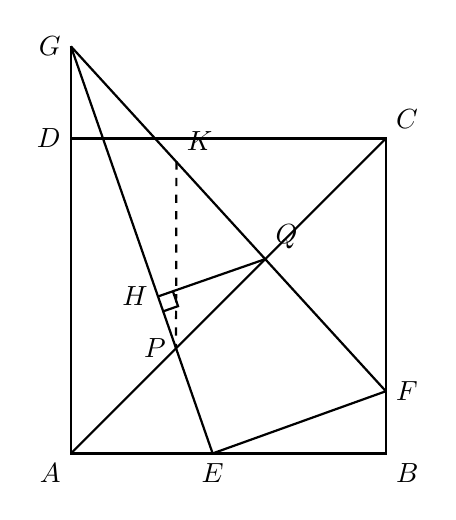
\begin{tikzpicture}[thick, scale=1]

  % 基本点
  \coordinate (A) at (0,0);
  \coordinate (B) at (4,0);
  \coordinate (C) at (4,4);
  \coordinate (D) at (0,4);
  \coordinate (G) at (0,5.17);
  \coordinate (E) at (1.8,0);
  \coordinate (F) at (4,0.79);
  \coordinate (K) at (1.34,3.71);

  % 交点 P、Q（路径相交）
  \path [name path=GE] (G) -- (E);
  \path [name path=GF] (G) -- (F);
  \path [name path=AC] (A) -- (C);
  \path [name intersections={of=GE and AC, by=P}];
  \path [name intersections={of=GF and AC, by=Q}];

  % 垂足 H：Q 到直线 EG 的投影
  \coordinate (H) at ($(E)!(Q)!(G)$);

  % 正方形 ABCD
  \draw (A) -- (B) -- (C) -- (D) -- cycle;

  % 左侧竖线 GA
  \draw (G) -- (A);

  % 其余线段
  \draw (G) -- (E);
  \draw (G) -- (F);
  \draw (A) -- (C);
  \draw (E) -- (F);
  \draw[dashed] (K) -- (P);

  % 新增线段 QH 与直角标记
  \draw (Q) -- (H);
  \draw pic[draw, angle radius=0.2cm] {right angle=Q--H--E};

  % 标签
  \node[left]        at (G) {$G$};
  \node[left]        at (D) {$D$};
  \node[above right] at (C) {$C$};
  \node[above right] at (K) {$K$};
  \node[above right] at (Q) {$Q$};
  \node[left]        at (P) {$P$};
  \node[below]       at (E) {$E$};
  \node[right]       at (F) {$F$};
  \node[below left]  at (A) {$A$};
  \node[below right] at (B) {$B$};
  \node[left]        at (H) {$H$};

\end{tikzpicture}
\end{document}
